\documentclass[twoside]{book}

% Packages required by doxygen
\usepackage{fixltx2e}
\usepackage{calc}
\usepackage{doxygen}
\usepackage[export]{adjustbox} % also loads graphicx
\usepackage{graphicx}
\usepackage[utf8]{inputenc}
\usepackage{makeidx}
\usepackage{multicol}
\usepackage{multirow}
\PassOptionsToPackage{warn}{textcomp}
\usepackage{textcomp}
\usepackage[nointegrals]{wasysym}
\usepackage[table]{xcolor}

% Font selection
\usepackage[T1]{fontenc}
\usepackage[scaled=.90]{helvet}
\usepackage{courier}
\usepackage{amssymb}
\usepackage{sectsty}
\renewcommand{\familydefault}{\sfdefault}
\allsectionsfont{%
  \fontseries{bc}\selectfont%
  \color{darkgray}%
}
\renewcommand{\DoxyLabelFont}{%
  \fontseries{bc}\selectfont%
  \color{darkgray}%
}
\newcommand{\+}{\discretionary{\mbox{\scriptsize$\hookleftarrow$}}{}{}}

% Page & text layout
\usepackage{geometry}
\geometry{%
  a4paper,%
  top=2.5cm,%
  bottom=2.5cm,%
  left=2.5cm,%
  right=2.5cm%
}
\tolerance=750
\hfuzz=15pt
\hbadness=750
\setlength{\emergencystretch}{15pt}
\setlength{\parindent}{0cm}
\setlength{\parskip}{0.2cm}
\makeatletter
\renewcommand{\paragraph}{%
  \@startsection{paragraph}{4}{0ex}{-1.0ex}{1.0ex}{%
    \normalfont\normalsize\bfseries\SS@parafont%
  }%
}
\renewcommand{\subparagraph}{%
  \@startsection{subparagraph}{5}{0ex}{-1.0ex}{1.0ex}{%
    \normalfont\normalsize\bfseries\SS@subparafont%
  }%
}
\makeatother

% Headers & footers
\usepackage{fancyhdr}
\pagestyle{fancyplain}
\fancyhead[LE]{\fancyplain{}{\bfseries\thepage}}
\fancyhead[CE]{\fancyplain{}{}}
\fancyhead[RE]{\fancyplain{}{\bfseries\leftmark}}
\fancyhead[LO]{\fancyplain{}{\bfseries\rightmark}}
\fancyhead[CO]{\fancyplain{}{}}
\fancyhead[RO]{\fancyplain{}{\bfseries\thepage}}
\fancyfoot[LE]{\fancyplain{}{}}
\fancyfoot[CE]{\fancyplain{}{}}
\fancyfoot[RE]{\fancyplain{}{\bfseries\scriptsize Generated on Thu Mar 26 2015 11\+:40\+:47 for Quiz\+Creator by Doxygen }}
\fancyfoot[LO]{\fancyplain{}{\bfseries\scriptsize Generated on Thu Mar 26 2015 11\+:40\+:47 for Quiz\+Creator by Doxygen }}
\fancyfoot[CO]{\fancyplain{}{}}
\fancyfoot[RO]{\fancyplain{}{}}
\renewcommand{\footrulewidth}{0.4pt}
\renewcommand{\chaptermark}[1]{%
  \markboth{#1}{}%
}
\renewcommand{\sectionmark}[1]{%
  \markright{\thesection\ #1}%
}

% Indices & bibliography
\usepackage{natbib}
\usepackage[titles]{tocloft}
\setcounter{tocdepth}{3}
\setcounter{secnumdepth}{5}
\makeindex

% Hyperlinks (required, but should be loaded last)
\usepackage{ifpdf}
\ifpdf
  \usepackage[pdftex,pagebackref=true]{hyperref}
\else
  \usepackage[ps2pdf,pagebackref=true]{hyperref}
\fi
\hypersetup{%
  colorlinks=true,%
  linkcolor=blue,%
  citecolor=blue,%
  unicode%
}

% Custom commands
\newcommand{\clearemptydoublepage}{%
  \newpage{\pagestyle{empty}\cleardoublepage}%
}


%===== C O N T E N T S =====

\begin{document}

% Titlepage & ToC
\hypersetup{pageanchor=false,
             bookmarks=true,
             bookmarksnumbered=true,
             pdfencoding=unicode
            }
\pagenumbering{roman}
\begin{titlepage}
\vspace*{7cm}
\begin{center}%
{\Large Quiz\+Creator }\\
\vspace*{1cm}
{\large Generated by Doxygen 1.8.9.1}\\
\vspace*{0.5cm}
{\small Thu Mar 26 2015 11:40:47}\\
\end{center}
\end{titlepage}
\clearemptydoublepage
\tableofcontents
\clearemptydoublepage
\pagenumbering{arabic}
\hypersetup{pageanchor=true}

%--- Begin generated contents ---
\chapter{Namespace Index}
\section{Packages}
Here are the packages with brief descriptions (if available)\+:\begin{DoxyCompactList}
\item\contentsline{section}{\hyperlink{namespace_website}{Website} }{\pageref{namespace_website}}{}
\end{DoxyCompactList}

\chapter{Hierarchical Index}
\section{Class Hierarchy}
This inheritance list is sorted roughly, but not completely, alphabetically\+:\begin{DoxyCompactList}
\item \contentsline{section}{Website.\+Models.\+Answer}{\pageref{class_website_1_1_models_1_1_answer}}{}
\item \contentsline{section}{Website.\+Models.\+Answer\+Quiz\+Log}{\pageref{class_website_1_1_models_1_1_answer_quiz_log}}{}
\item Api\+Controller\begin{DoxyCompactList}
\item \contentsline{section}{Website.\+Controllers.\+Login\+Controller}{\pageref{class_website_1_1_controllers_1_1_login_controller}}{}
\end{DoxyCompactList}
\item \contentsline{section}{Website.\+Asp\+Net\+Roles}{\pageref{class_website_1_1_asp_net_roles}}{}
\item \contentsline{section}{Website.\+Asp\+Net\+User\+Claims}{\pageref{class_website_1_1_asp_net_user_claims}}{}
\item \contentsline{section}{Website.\+Asp\+Net\+User\+Logins}{\pageref{class_website_1_1_asp_net_user_logins}}{}
\item \contentsline{section}{Website.\+Asp\+Net\+Users}{\pageref{class_website_1_1_asp_net_users}}{}
\item \contentsline{section}{Website.\+Bundle\+Config}{\pageref{class_website_1_1_bundle_config}}{}
\item Controller\begin{DoxyCompactList}
\item \contentsline{section}{Website.\+Controllers.\+Answer\+Quiz\+Controller}{\pageref{class_website_1_1_controllers_1_1_answer_quiz_controller}}{}
\item \contentsline{section}{Website.\+Controllers.\+Config\+Group\+Controller}{\pageref{class_website_1_1_controllers_1_1_config_group_controller}}{}
\item \contentsline{section}{Website.\+Controllers.\+Config\+Quizzes\+Controller}{\pageref{class_website_1_1_controllers_1_1_config_quizzes_controller}}{}
\item \contentsline{section}{Website.\+Controllers.\+Create\+Quiz\+Controller}{\pageref{class_website_1_1_controllers_1_1_create_quiz_controller}}{}
\item \contentsline{section}{Website.\+Controllers.\+Create\+User\+Controller}{\pageref{class_website_1_1_controllers_1_1_create_user_controller}}{}
\item \contentsline{section}{Website.\+Controllers.\+Favorites\+Controller}{\pageref{class_website_1_1_controllers_1_1_favorites_controller}}{}
\item \contentsline{section}{Website.\+Controllers.\+Find\+Quiz\+Controller}{\pageref{class_website_1_1_controllers_1_1_find_quiz_controller}}{}
\item \contentsline{section}{Website.\+Controllers.\+Group\+Controller}{\pageref{class_website_1_1_controllers_1_1_group_controller}}{}
\item \contentsline{section}{Website.\+Controllers.\+Home\+Controller}{\pageref{class_website_1_1_controllers_1_1_home_controller}}{}
\item \contentsline{section}{Website.\+Controllers.\+Validation\+Controller}{\pageref{class_website_1_1_controllers_1_1_validation_controller}}{}
\end{DoxyCompactList}
\item Db\+Context\begin{DoxyCompactList}
\item \contentsline{section}{Website.\+Models.\+Quiz\+Creator\+Context}{\pageref{class_website_1_1_models_1_1_quiz_creator_context}}{}
\end{DoxyCompactList}
\item Db\+Migration\begin{DoxyCompactList}
\item \contentsline{section}{Website.\+Migrations.\+Added\+\_\+\+Answer\+Quiz\+Log}{\pageref{class_website_1_1_migrations_1_1_added___answer_quiz_log}}{}
\item \contentsline{section}{Website.\+Migrations.\+added\+\_\+tags\+\_\+to\+\_\+groups\+\_\+many\+\_\+to\+\_\+many}{\pageref{class_website_1_1_migrations_1_1added__tags__to__groups__many__to__many}}{}
\item \contentsline{section}{Website.\+Migrations.\+Added\+Active\+To\+Quiz}{\pageref{class_website_1_1_migrations_1_1_added_active_to_quiz}}{}
\item \contentsline{section}{Website.\+Migrations.\+Added\+Favoritemodelandlistoffavoritesto\+Asp\+Net\+Users}{\pageref{class_website_1_1_migrations_1_1_added_favoritemodelandlistoffavoritesto_asp_net_users}}{}
\item \contentsline{section}{Website.\+Migrations.\+Added\+Filepath\+To\+Question}{\pageref{class_website_1_1_migrations_1_1_added_filepath_to_question}}{}
\item \contentsline{section}{Website.\+Migrations.\+Addedfirstnameoglastnameto\+Asp\+Net\+Users}{\pageref{class_website_1_1_migrations_1_1_addedfirstnameoglastnameto_asp_net_users}}{}
\item \contentsline{section}{Website.\+Migrations.\+added\+Id\+References\+To\+User\+And\+Answers\+In\+Answer\+Quiz\+Log}{\pageref{class_website_1_1_migrations_1_1added_id_references_to_user_and_answers_in_answer_quiz_log}}{}
\item \contentsline{section}{Website.\+Migrations.\+Added\+Points\+To\+Answer}{\pageref{class_website_1_1_migrations_1_1_added_points_to_answer}}{}
\item \contentsline{section}{Website.\+Migrations.\+Addeduser\+I\+Danduserreferenceto\+Quizmodel}{\pageref{class_website_1_1_migrations_1_1_addeduser_i_danduserreferenceto_quizmodel}}{}
\item \contentsline{section}{Website.\+Migrations.\+addnewtable}{\pageref{class_website_1_1_migrations_1_1addnewtable}}{}
\item \contentsline{section}{Website.\+Migrations.\+add\+Q}{\pageref{class_website_1_1_migrations_1_1add_q}}{}
\item \contentsline{section}{Website.\+Migrations.\+add\+Q1}{\pageref{class_website_1_1_migrations_1_1add_q1}}{}
\item \contentsline{section}{Website.\+Migrations.\+addquiz}{\pageref{class_website_1_1_migrations_1_1addquiz}}{}
\item \contentsline{section}{Website.\+Migrations.\+addquiz1}{\pageref{class_website_1_1_migrations_1_1addquiz1}}{}
\item \contentsline{section}{Website.\+Migrations.\+Anotherchangeagain}{\pageref{class_website_1_1_migrations_1_1_anotherchangeagain}}{}
\item \contentsline{section}{Website.\+Migrations.\+changed\+\_\+\+Reference\+\_\+\+Answer\+Quiz\+Log\+\_\+\+Asp\+Net\+Users\+Id\+\_\+\+To\+\_\+\+String}{\pageref{class_website_1_1_migrations_1_1changed___reference___answer_quiz_log___asp_net_users_id___to___string}}{}
\item \contentsline{section}{Website.\+Migrations.\+changed\+Pending\+Apparantly}{\pageref{class_website_1_1_migrations_1_1changed_pending_apparantly}}{}
\item \contentsline{section}{Website.\+Migrations.\+Group\+\_\+requirement\+\_\+changed}{\pageref{class_website_1_1_migrations_1_1_group__requirement__changed}}{}
\item \contentsline{section}{Website.\+Migrations.\+Groups\+\_\+added}{\pageref{class_website_1_1_migrations_1_1_groups__added}}{}
\item \contentsline{section}{Website.\+Migrations.\+mangler\+\_\+noget}{\pageref{class_website_1_1_migrations_1_1mangler__noget}}{}
\item \contentsline{section}{Website.\+Migrations.\+nyt\+Question}{\pageref{class_website_1_1_migrations_1_1nyt_question}}{}
\item \contentsline{section}{Website.\+Migrations.\+nyt\+Question1}{\pageref{class_website_1_1_migrations_1_1nyt_question1}}{}
\item \contentsline{section}{Website.\+Migrations.\+nyt\+Question2}{\pageref{class_website_1_1_migrations_1_1nyt_question2}}{}
\item \contentsline{section}{Website.\+Migrations.\+nyt\+Question3}{\pageref{class_website_1_1_migrations_1_1nyt_question3}}{}
\item \contentsline{section}{Website.\+Migrations.\+nyt\+Question4}{\pageref{class_website_1_1_migrations_1_1nyt_question4}}{}
\item \contentsline{section}{Website.\+Migrations.\+nyt\+Question5}{\pageref{class_website_1_1_migrations_1_1nyt_question5}}{}
\item \contentsline{section}{Website.\+Migrations.\+nyt\+Question6}{\pageref{class_website_1_1_migrations_1_1nyt_question6}}{}
\item \contentsline{section}{Website.\+Migrations.\+oohagain}{\pageref{class_website_1_1_migrations_1_1oohagain}}{}
\item \contentsline{section}{Website.\+Migrations.\+questionadd}{\pageref{class_website_1_1_migrations_1_1questionadd}}{}
\item \contentsline{section}{Website.\+Migrations.\+questionadd1}{\pageref{class_website_1_1_migrations_1_1questionadd1}}{}
\item \contentsline{section}{Website.\+Migrations.\+questionadd2}{\pageref{class_website_1_1_migrations_1_1questionadd2}}{}
\item \contentsline{section}{Website.\+Migrations.\+questionadd3}{\pageref{class_website_1_1_migrations_1_1questionadd3}}{}
\item \contentsline{section}{Website.\+Migrations.\+questionadd4}{\pageref{class_website_1_1_migrations_1_1questionadd4}}{}
\item \contentsline{section}{Website.\+Migrations.\+questionadd5}{\pageref{class_website_1_1_migrations_1_1questionadd5}}{}
\item \contentsline{section}{Website.\+Migrations.\+Remote\+\_\+validation\+\_\+in\+\_\+group\+Name}{\pageref{class_website_1_1_migrations_1_1_remote__validation__in__group_name}}{}
\item \contentsline{section}{Website.\+Migrations.\+Removed\+File\+Path\+Table\+\_\+\+Added\+File\+Path\+To\+Question}{\pageref{class_website_1_1_migrations_1_1_removed_file_path_table___added_file_path_to_question}}{}
\item \contentsline{section}{Website.\+Migrations.\+Removed\+Required\+For\+Active\+In\+Quiz}{\pageref{class_website_1_1_migrations_1_1_removed_required_for_active_in_quiz}}{}
\item \contentsline{section}{Website.\+Migrations.\+removed\+Required\+From\+User\+In\+Answer\+Quiz\+Log}{\pageref{class_website_1_1_migrations_1_1removed_required_from_user_in_answer_quiz_log}}{}
\item \contentsline{section}{Website.\+Migrations.\+Removing\+\_\+requirements\+\_\+to\+Last\+\_\+and\+\_\+firstname}{\pageref{class_website_1_1_migrations_1_1_removing__requirements__to_last__and__firstname}}{}
\item \contentsline{section}{Website.\+Migrations.\+Seperated\+Favorites}{\pageref{class_website_1_1_migrations_1_1_seperated_favorites}}{}
\item \contentsline{section}{Website.\+Migrations.\+Some\+Change\+Idid}{\pageref{class_website_1_1_migrations_1_1_some_change_idid}}{}
\item \contentsline{section}{Website.\+Migrations.\+Somechangeto\+Quiz}{\pageref{class_website_1_1_migrations_1_1_somechangeto_quiz}}{}
\item \contentsline{section}{Website.\+Migrations.\+updating\+\_\+\+Group\+\_\+entity}{\pageref{class_website_1_1_migrations_1_1updating___group__entity}}{}
\item \contentsline{section}{Website.\+Migrations.\+updatinging\+S\+Um\+Changes}{\pageref{class_website_1_1_migrations_1_1updatinging_s_um_changes}}{}
\item \contentsline{section}{Website.\+Migrations.\+x}{\pageref{class_website_1_1_migrations_1_1x}}{}
\item \contentsline{section}{Website.\+Migrations.\+x1}{\pageref{class_website_1_1_migrations_1_1x1}}{}
\item \contentsline{section}{Website.\+Migrations.\+x10}{\pageref{class_website_1_1_migrations_1_1x10}}{}
\item \contentsline{section}{Website.\+Migrations.\+x11}{\pageref{class_website_1_1_migrations_1_1x11}}{}
\item \contentsline{section}{Website.\+Migrations.\+x12}{\pageref{class_website_1_1_migrations_1_1x12}}{}
\item \contentsline{section}{Website.\+Migrations.\+x13}{\pageref{class_website_1_1_migrations_1_1x13}}{}
\item \contentsline{section}{Website.\+Migrations.\+x14}{\pageref{class_website_1_1_migrations_1_1x14}}{}
\item \contentsline{section}{Website.\+Migrations.\+x15}{\pageref{class_website_1_1_migrations_1_1x15}}{}
\item \contentsline{section}{Website.\+Migrations.\+x16}{\pageref{class_website_1_1_migrations_1_1x16}}{}
\item \contentsline{section}{Website.\+Migrations.\+x17}{\pageref{class_website_1_1_migrations_1_1x17}}{}
\item \contentsline{section}{Website.\+Migrations.\+x18}{\pageref{class_website_1_1_migrations_1_1x18}}{}
\item \contentsline{section}{Website.\+Migrations.\+x19}{\pageref{class_website_1_1_migrations_1_1x19}}{}
\item \contentsline{section}{Website.\+Migrations.\+x2}{\pageref{class_website_1_1_migrations_1_1x2}}{}
\item \contentsline{section}{Website.\+Migrations.\+x20}{\pageref{class_website_1_1_migrations_1_1x20}}{}
\item \contentsline{section}{Website.\+Migrations.\+x21}{\pageref{class_website_1_1_migrations_1_1x21}}{}
\item \contentsline{section}{Website.\+Migrations.\+x22}{\pageref{class_website_1_1_migrations_1_1x22}}{}
\item \contentsline{section}{Website.\+Migrations.\+x23}{\pageref{class_website_1_1_migrations_1_1x23}}{}
\item \contentsline{section}{Website.\+Migrations.\+x24}{\pageref{class_website_1_1_migrations_1_1x24}}{}
\item \contentsline{section}{Website.\+Migrations.\+x25}{\pageref{class_website_1_1_migrations_1_1x25}}{}
\item \contentsline{section}{Website.\+Migrations.\+x26}{\pageref{class_website_1_1_migrations_1_1x26}}{}
\item \contentsline{section}{Website.\+Migrations.\+x27}{\pageref{class_website_1_1_migrations_1_1x27}}{}
\item \contentsline{section}{Website.\+Migrations.\+x28}{\pageref{class_website_1_1_migrations_1_1x28}}{}
\item \contentsline{section}{Website.\+Migrations.\+x29}{\pageref{class_website_1_1_migrations_1_1x29}}{}
\item \contentsline{section}{Website.\+Migrations.\+x3}{\pageref{class_website_1_1_migrations_1_1x3}}{}
\item \contentsline{section}{Website.\+Migrations.\+x30}{\pageref{class_website_1_1_migrations_1_1x30}}{}
\item \contentsline{section}{Website.\+Migrations.\+x31}{\pageref{class_website_1_1_migrations_1_1x31}}{}
\item \contentsline{section}{Website.\+Migrations.\+x32}{\pageref{class_website_1_1_migrations_1_1x32}}{}
\item \contentsline{section}{Website.\+Migrations.\+x33}{\pageref{class_website_1_1_migrations_1_1x33}}{}
\item \contentsline{section}{Website.\+Migrations.\+x34}{\pageref{class_website_1_1_migrations_1_1x34}}{}
\item \contentsline{section}{Website.\+Migrations.\+x35}{\pageref{class_website_1_1_migrations_1_1x35}}{}
\item \contentsline{section}{Website.\+Migrations.\+x4}{\pageref{class_website_1_1_migrations_1_1x4}}{}
\item \contentsline{section}{Website.\+Migrations.\+x5}{\pageref{class_website_1_1_migrations_1_1x5}}{}
\item \contentsline{section}{Website.\+Migrations.\+x6}{\pageref{class_website_1_1_migrations_1_1x6}}{}
\item \contentsline{section}{Website.\+Migrations.\+x7}{\pageref{class_website_1_1_migrations_1_1x7}}{}
\item \contentsline{section}{Website.\+Migrations.\+x8}{\pageref{class_website_1_1_migrations_1_1x8}}{}
\item \contentsline{section}{Website.\+Migrations.\+x9}{\pageref{class_website_1_1_migrations_1_1x9}}{}
\end{DoxyCompactList}
\item Exception\begin{DoxyCompactList}
\item \contentsline{section}{Website.\+Models.\+Incomplete\+Quiz\+Exception}{\pageref{class_website_1_1_models_1_1_incomplete_quiz_exception}}{}
\item \contentsline{section}{Website.\+Models.\+No\+Answer\+Found\+Exception}{\pageref{class_website_1_1_models_1_1_no_answer_found_exception}}{}
\item \contentsline{section}{Website.\+Models.\+No\+Answers\+Found\+Exception}{\pageref{class_website_1_1_models_1_1_no_answers_found_exception}}{}
\item \contentsline{section}{Website.\+Models.\+No\+Question\+Found\+Exception}{\pageref{class_website_1_1_models_1_1_no_question_found_exception}}{}
\item \contentsline{section}{Website.\+Models.\+Quiz\+Model\+Exception}{\pageref{class_website_1_1_models_1_1_quiz_model_exception}}{}
\item \contentsline{section}{Website.\+Models.\+User\+Rights\+Exception}{\pageref{class_website_1_1_models_1_1_user_rights_exception}}{}
\end{DoxyCompactList}
\item \contentsline{section}{Website.\+Models.\+Favorite\+Group}{\pageref{class_website_1_1_models_1_1_favorite_group}}{}
\item \contentsline{section}{Website.\+Models.\+Favorite\+Quiz}{\pageref{class_website_1_1_models_1_1_favorite_quiz}}{}
\item \contentsline{section}{Website.\+Filter\+Config}{\pageref{class_website_1_1_filter_config}}{}
\item \contentsline{section}{Website.\+Models.\+Group}{\pageref{class_website_1_1_models_1_1_group}}{}
\item Http\+Application\begin{DoxyCompactList}
\item \contentsline{section}{Website.\+Mvc\+Application}{\pageref{class_website_1_1_mvc_application}}{}
\end{DoxyCompactList}
\item \contentsline{section}{Website.\+Models.\+I\+D\+A\+L\+E\+F}{\pageref{interface_website_1_1_models_1_1_i_d_a_l_e_f}}{}
\begin{DoxyCompactList}
\item \contentsline{section}{Website.\+Models.\+D\+A\+L\+E\+F}{\pageref{class_website_1_1_models_1_1_d_a_l_e_f}}{}
\end{DoxyCompactList}
\item I\+Migration\+Metadata\begin{DoxyCompactList}
\item \contentsline{section}{Website.\+Migrations.\+Added\+\_\+\+Answer\+Quiz\+Log}{\pageref{class_website_1_1_migrations_1_1_added___answer_quiz_log}}{}
\item \contentsline{section}{Website.\+Migrations.\+added\+\_\+tags\+\_\+to\+\_\+groups\+\_\+many\+\_\+to\+\_\+many}{\pageref{class_website_1_1_migrations_1_1added__tags__to__groups__many__to__many}}{}
\item \contentsline{section}{Website.\+Migrations.\+Added\+Active\+To\+Quiz}{\pageref{class_website_1_1_migrations_1_1_added_active_to_quiz}}{}
\item \contentsline{section}{Website.\+Migrations.\+Added\+Favoritemodelandlistoffavoritesto\+Asp\+Net\+Users}{\pageref{class_website_1_1_migrations_1_1_added_favoritemodelandlistoffavoritesto_asp_net_users}}{}
\item \contentsline{section}{Website.\+Migrations.\+Added\+Filepath\+To\+Question}{\pageref{class_website_1_1_migrations_1_1_added_filepath_to_question}}{}
\item \contentsline{section}{Website.\+Migrations.\+Addedfirstnameoglastnameto\+Asp\+Net\+Users}{\pageref{class_website_1_1_migrations_1_1_addedfirstnameoglastnameto_asp_net_users}}{}
\item \contentsline{section}{Website.\+Migrations.\+added\+Id\+References\+To\+User\+And\+Answers\+In\+Answer\+Quiz\+Log}{\pageref{class_website_1_1_migrations_1_1added_id_references_to_user_and_answers_in_answer_quiz_log}}{}
\item \contentsline{section}{Website.\+Migrations.\+Added\+Points\+To\+Answer}{\pageref{class_website_1_1_migrations_1_1_added_points_to_answer}}{}
\item \contentsline{section}{Website.\+Migrations.\+Addeduser\+I\+Danduserreferenceto\+Quizmodel}{\pageref{class_website_1_1_migrations_1_1_addeduser_i_danduserreferenceto_quizmodel}}{}
\item \contentsline{section}{Website.\+Migrations.\+addnewtable}{\pageref{class_website_1_1_migrations_1_1addnewtable}}{}
\item \contentsline{section}{Website.\+Migrations.\+add\+Q}{\pageref{class_website_1_1_migrations_1_1add_q}}{}
\item \contentsline{section}{Website.\+Migrations.\+add\+Q1}{\pageref{class_website_1_1_migrations_1_1add_q1}}{}
\item \contentsline{section}{Website.\+Migrations.\+addquiz}{\pageref{class_website_1_1_migrations_1_1addquiz}}{}
\item \contentsline{section}{Website.\+Migrations.\+addquiz1}{\pageref{class_website_1_1_migrations_1_1addquiz1}}{}
\item \contentsline{section}{Website.\+Migrations.\+Anotherchangeagain}{\pageref{class_website_1_1_migrations_1_1_anotherchangeagain}}{}
\item \contentsline{section}{Website.\+Migrations.\+changed\+\_\+\+Reference\+\_\+\+Answer\+Quiz\+Log\+\_\+\+Asp\+Net\+Users\+Id\+\_\+\+To\+\_\+\+String}{\pageref{class_website_1_1_migrations_1_1changed___reference___answer_quiz_log___asp_net_users_id___to___string}}{}
\item \contentsline{section}{Website.\+Migrations.\+changed\+Pending\+Apparantly}{\pageref{class_website_1_1_migrations_1_1changed_pending_apparantly}}{}
\item \contentsline{section}{Website.\+Migrations.\+Group\+\_\+requirement\+\_\+changed}{\pageref{class_website_1_1_migrations_1_1_group__requirement__changed}}{}
\item \contentsline{section}{Website.\+Migrations.\+Groups\+\_\+added}{\pageref{class_website_1_1_migrations_1_1_groups__added}}{}
\item \contentsline{section}{Website.\+Migrations.\+mangler\+\_\+noget}{\pageref{class_website_1_1_migrations_1_1mangler__noget}}{}
\item \contentsline{section}{Website.\+Migrations.\+nyt\+Question}{\pageref{class_website_1_1_migrations_1_1nyt_question}}{}
\item \contentsline{section}{Website.\+Migrations.\+nyt\+Question1}{\pageref{class_website_1_1_migrations_1_1nyt_question1}}{}
\item \contentsline{section}{Website.\+Migrations.\+nyt\+Question2}{\pageref{class_website_1_1_migrations_1_1nyt_question2}}{}
\item \contentsline{section}{Website.\+Migrations.\+nyt\+Question3}{\pageref{class_website_1_1_migrations_1_1nyt_question3}}{}
\item \contentsline{section}{Website.\+Migrations.\+nyt\+Question4}{\pageref{class_website_1_1_migrations_1_1nyt_question4}}{}
\item \contentsline{section}{Website.\+Migrations.\+nyt\+Question5}{\pageref{class_website_1_1_migrations_1_1nyt_question5}}{}
\item \contentsline{section}{Website.\+Migrations.\+nyt\+Question6}{\pageref{class_website_1_1_migrations_1_1nyt_question6}}{}
\item \contentsline{section}{Website.\+Migrations.\+oohagain}{\pageref{class_website_1_1_migrations_1_1oohagain}}{}
\item \contentsline{section}{Website.\+Migrations.\+questionadd}{\pageref{class_website_1_1_migrations_1_1questionadd}}{}
\item \contentsline{section}{Website.\+Migrations.\+questionadd1}{\pageref{class_website_1_1_migrations_1_1questionadd1}}{}
\item \contentsline{section}{Website.\+Migrations.\+questionadd2}{\pageref{class_website_1_1_migrations_1_1questionadd2}}{}
\item \contentsline{section}{Website.\+Migrations.\+questionadd3}{\pageref{class_website_1_1_migrations_1_1questionadd3}}{}
\item \contentsline{section}{Website.\+Migrations.\+questionadd4}{\pageref{class_website_1_1_migrations_1_1questionadd4}}{}
\item \contentsline{section}{Website.\+Migrations.\+questionadd5}{\pageref{class_website_1_1_migrations_1_1questionadd5}}{}
\item \contentsline{section}{Website.\+Migrations.\+Remote\+\_\+validation\+\_\+in\+\_\+group\+Name}{\pageref{class_website_1_1_migrations_1_1_remote__validation__in__group_name}}{}
\item \contentsline{section}{Website.\+Migrations.\+Removed\+File\+Path\+Table\+\_\+\+Added\+File\+Path\+To\+Question}{\pageref{class_website_1_1_migrations_1_1_removed_file_path_table___added_file_path_to_question}}{}
\item \contentsline{section}{Website.\+Migrations.\+Removed\+Required\+For\+Active\+In\+Quiz}{\pageref{class_website_1_1_migrations_1_1_removed_required_for_active_in_quiz}}{}
\item \contentsline{section}{Website.\+Migrations.\+removed\+Required\+From\+User\+In\+Answer\+Quiz\+Log}{\pageref{class_website_1_1_migrations_1_1removed_required_from_user_in_answer_quiz_log}}{}
\item \contentsline{section}{Website.\+Migrations.\+Removing\+\_\+requirements\+\_\+to\+Last\+\_\+and\+\_\+firstname}{\pageref{class_website_1_1_migrations_1_1_removing__requirements__to_last__and__firstname}}{}
\item \contentsline{section}{Website.\+Migrations.\+Seperated\+Favorites}{\pageref{class_website_1_1_migrations_1_1_seperated_favorites}}{}
\item \contentsline{section}{Website.\+Migrations.\+Some\+Change\+Idid}{\pageref{class_website_1_1_migrations_1_1_some_change_idid}}{}
\item \contentsline{section}{Website.\+Migrations.\+Somechangeto\+Quiz}{\pageref{class_website_1_1_migrations_1_1_somechangeto_quiz}}{}
\item \contentsline{section}{Website.\+Migrations.\+updating\+\_\+\+Group\+\_\+entity}{\pageref{class_website_1_1_migrations_1_1updating___group__entity}}{}
\item \contentsline{section}{Website.\+Migrations.\+updatinging\+S\+Um\+Changes}{\pageref{class_website_1_1_migrations_1_1updatinging_s_um_changes}}{}
\item \contentsline{section}{Website.\+Migrations.\+x}{\pageref{class_website_1_1_migrations_1_1x}}{}
\item \contentsline{section}{Website.\+Migrations.\+x1}{\pageref{class_website_1_1_migrations_1_1x1}}{}
\item \contentsline{section}{Website.\+Migrations.\+x10}{\pageref{class_website_1_1_migrations_1_1x10}}{}
\item \contentsline{section}{Website.\+Migrations.\+x11}{\pageref{class_website_1_1_migrations_1_1x11}}{}
\item \contentsline{section}{Website.\+Migrations.\+x12}{\pageref{class_website_1_1_migrations_1_1x12}}{}
\item \contentsline{section}{Website.\+Migrations.\+x13}{\pageref{class_website_1_1_migrations_1_1x13}}{}
\item \contentsline{section}{Website.\+Migrations.\+x14}{\pageref{class_website_1_1_migrations_1_1x14}}{}
\item \contentsline{section}{Website.\+Migrations.\+x15}{\pageref{class_website_1_1_migrations_1_1x15}}{}
\item \contentsline{section}{Website.\+Migrations.\+x16}{\pageref{class_website_1_1_migrations_1_1x16}}{}
\item \contentsline{section}{Website.\+Migrations.\+x17}{\pageref{class_website_1_1_migrations_1_1x17}}{}
\item \contentsline{section}{Website.\+Migrations.\+x18}{\pageref{class_website_1_1_migrations_1_1x18}}{}
\item \contentsline{section}{Website.\+Migrations.\+x19}{\pageref{class_website_1_1_migrations_1_1x19}}{}
\item \contentsline{section}{Website.\+Migrations.\+x2}{\pageref{class_website_1_1_migrations_1_1x2}}{}
\item \contentsline{section}{Website.\+Migrations.\+x20}{\pageref{class_website_1_1_migrations_1_1x20}}{}
\item \contentsline{section}{Website.\+Migrations.\+x21}{\pageref{class_website_1_1_migrations_1_1x21}}{}
\item \contentsline{section}{Website.\+Migrations.\+x22}{\pageref{class_website_1_1_migrations_1_1x22}}{}
\item \contentsline{section}{Website.\+Migrations.\+x23}{\pageref{class_website_1_1_migrations_1_1x23}}{}
\item \contentsline{section}{Website.\+Migrations.\+x24}{\pageref{class_website_1_1_migrations_1_1x24}}{}
\item \contentsline{section}{Website.\+Migrations.\+x25}{\pageref{class_website_1_1_migrations_1_1x25}}{}
\item \contentsline{section}{Website.\+Migrations.\+x26}{\pageref{class_website_1_1_migrations_1_1x26}}{}
\item \contentsline{section}{Website.\+Migrations.\+x27}{\pageref{class_website_1_1_migrations_1_1x27}}{}
\item \contentsline{section}{Website.\+Migrations.\+x28}{\pageref{class_website_1_1_migrations_1_1x28}}{}
\item \contentsline{section}{Website.\+Migrations.\+x29}{\pageref{class_website_1_1_migrations_1_1x29}}{}
\item \contentsline{section}{Website.\+Migrations.\+x3}{\pageref{class_website_1_1_migrations_1_1x3}}{}
\item \contentsline{section}{Website.\+Migrations.\+x30}{\pageref{class_website_1_1_migrations_1_1x30}}{}
\item \contentsline{section}{Website.\+Migrations.\+x31}{\pageref{class_website_1_1_migrations_1_1x31}}{}
\item \contentsline{section}{Website.\+Migrations.\+x32}{\pageref{class_website_1_1_migrations_1_1x32}}{}
\item \contentsline{section}{Website.\+Migrations.\+x33}{\pageref{class_website_1_1_migrations_1_1x33}}{}
\item \contentsline{section}{Website.\+Migrations.\+x34}{\pageref{class_website_1_1_migrations_1_1x34}}{}
\item \contentsline{section}{Website.\+Migrations.\+x35}{\pageref{class_website_1_1_migrations_1_1x35}}{}
\item \contentsline{section}{Website.\+Migrations.\+x4}{\pageref{class_website_1_1_migrations_1_1x4}}{}
\item \contentsline{section}{Website.\+Migrations.\+x5}{\pageref{class_website_1_1_migrations_1_1x5}}{}
\item \contentsline{section}{Website.\+Migrations.\+x6}{\pageref{class_website_1_1_migrations_1_1x6}}{}
\item \contentsline{section}{Website.\+Migrations.\+x7}{\pageref{class_website_1_1_migrations_1_1x7}}{}
\item \contentsline{section}{Website.\+Migrations.\+x8}{\pageref{class_website_1_1_migrations_1_1x8}}{}
\item \contentsline{section}{Website.\+Migrations.\+x9}{\pageref{class_website_1_1_migrations_1_1x9}}{}
\end{DoxyCompactList}
\item \contentsline{section}{Website.\+Controllers.\+I\+Quiz\+Model}{\pageref{interface_website_1_1_controllers_1_1_i_quiz_model}}{}
\begin{DoxyCompactList}
\item \contentsline{section}{Website.\+Models.\+Quiz\+Model}{\pageref{class_website_1_1_models_1_1_quiz_model}}{}
\end{DoxyCompactList}
\item Page\begin{DoxyCompactList}
\item \contentsline{section}{Website.\+Register}{\pageref{class_website_1_1_register}}{}
\end{DoxyCompactList}
\item \contentsline{section}{Website.\+Models.\+Question}{\pageref{class_website_1_1_models_1_1_question}}{}
\item \contentsline{section}{Website.\+Models.\+Quiz}{\pageref{class_website_1_1_models_1_1_quiz}}{}
\item \contentsline{section}{Website.\+Route\+Config}{\pageref{class_website_1_1_route_config}}{}
\item \contentsline{section}{Website.\+Startup}{\pageref{class_website_1_1_startup}}{}
\item \contentsline{section}{Website.\+Models.\+Tag}{\pageref{class_website_1_1_models_1_1_tag}}{}
\item \contentsline{section}{Website.\+Controllers.\+temp\+User}{\pageref{class_website_1_1_controllers_1_1temp_user}}{}
\end{DoxyCompactList}

\chapter{Class Index}
\section{Class List}
Here are the classes, structs, unions and interfaces with brief descriptions\+:\begin{DoxyCompactList}
\item\contentsline{section}{\hyperlink{class_website_1_1_mvc_application}{Website.\+Mvc\+Application} }{\pageref{class_website_1_1_mvc_application}}{}
\item\contentsline{section}{\hyperlink{class_website_1_1_startup}{Website.\+Startup} }{\pageref{class_website_1_1_startup}}{}
\end{DoxyCompactList}

\chapter{Namespace Documentation}
\hypertarget{namespace_website}{}\section{Package Website}
\label{namespace_website}\index{Website@{Website}}
\subsection*{Namespaces}
\begin{DoxyCompactItemize}
\item 
package \hyperlink{namespace_website_1_1_controllers}{Controllers}
\item 
package \hyperlink{namespace_website_1_1_migrations}{Migrations}
\item 
package \hyperlink{namespace_website_1_1_models}{Models}
\end{DoxyCompactItemize}
\subsection*{Classes}
\begin{DoxyCompactItemize}
\item 
class \hyperlink{class_website_1_1_asp_net_roles}{Asp\+Net\+Roles}
\item 
class \hyperlink{class_website_1_1_asp_net_user_claims}{Asp\+Net\+User\+Claims}
\item 
class \hyperlink{class_website_1_1_asp_net_user_logins}{Asp\+Net\+User\+Logins}
\item 
class \hyperlink{class_website_1_1_asp_net_users}{Asp\+Net\+Users}
\item 
class \hyperlink{class_website_1_1_bundle_config}{Bundle\+Config}
\item 
class \hyperlink{class_website_1_1_filter_config}{Filter\+Config}
\item 
class \hyperlink{class_website_1_1_mvc_application}{Mvc\+Application}
\item 
class \hyperlink{class_website_1_1_register}{Register}
\item 
class \hyperlink{class_website_1_1_route_config}{Route\+Config}
\item 
class \hyperlink{class_website_1_1_startup}{Startup}
\item 
class {\bfseries Web\+Api\+Config}
\end{DoxyCompactItemize}

\chapter{Class Documentation}
\hypertarget{class_website_1_1_mvc_application}{}\section{Website.\+Mvc\+Application Class Reference}
\label{class_website_1_1_mvc_application}\index{Website.\+Mvc\+Application@{Website.\+Mvc\+Application}}
Inheritance diagram for Website.\+Mvc\+Application\+:\begin{figure}[H]
\begin{center}
\leavevmode
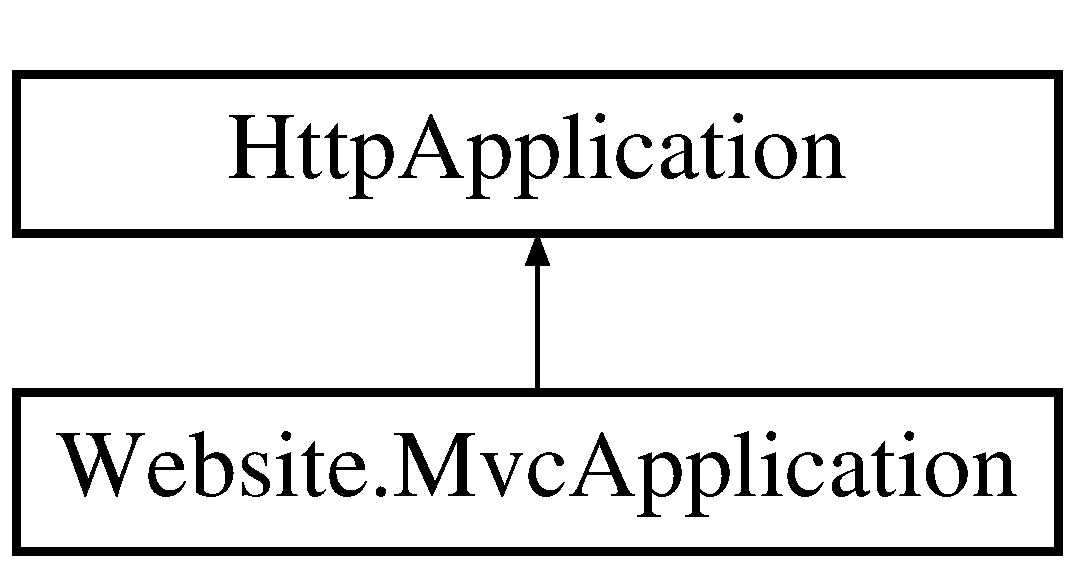
\includegraphics[height=2.000000cm]{class_website_1_1_mvc_application}
\end{center}
\end{figure}
\subsection*{Protected Member Functions}
\begin{DoxyCompactItemize}
\item 
\hypertarget{class_website_1_1_mvc_application_a6ee3215b20567a5b7903b837110d37dc}{}void {\bfseries Application\+\_\+\+Start} ()\label{class_website_1_1_mvc_application_a6ee3215b20567a5b7903b837110d37dc}

\end{DoxyCompactItemize}


The documentation for this class was generated from the following file\+:\begin{DoxyCompactItemize}
\item 
C\+:/\+Users/\+Lasse/\+Documents/\+M\+E\+G\+A/4. Semester/\+P\+R\+J/quizcreator/\+Website/Global.\+asax.\+cs\end{DoxyCompactItemize}

\hypertarget{class_website_1_1_startup}{}\section{Website.\+Startup Class Reference}
\label{class_website_1_1_startup}\index{Website.\+Startup@{Website.\+Startup}}
\subsection*{Public Member Functions}
\begin{DoxyCompactItemize}
\item 
\hypertarget{class_website_1_1_startup_a510c252a0bbe1235011e5f4fab7393b2}{}void {\bfseries Configuration} (I\+App\+Builder app)\label{class_website_1_1_startup_a510c252a0bbe1235011e5f4fab7393b2}

\end{DoxyCompactItemize}


The documentation for this class was generated from the following file\+:\begin{DoxyCompactItemize}
\item 
C\+:/\+Users/\+Lasse/\+Documents/\+M\+E\+G\+A/4. Semester/\+P\+R\+J/quizcreator/\+Website/Startup.\+cs\end{DoxyCompactItemize}

%--- End generated contents ---

% Index
\backmatter
\newpage
\phantomsection
\clearemptydoublepage
\addcontentsline{toc}{chapter}{Index}
\printindex

\end{document}
